\documentclass[]{DissertateUSU}
\usepackage{lmodern}
\usepackage{amssymb,amsmath}
\usepackage{ifxetex,ifluatex}
\usepackage{fixltx2e} % provides \textsubscript
\ifnum 0\ifxetex 1\fi\ifluatex 1\fi=0 % if pdftex
  \usepackage[T1]{fontenc}
  \usepackage[utf8]{inputenc}
\else % if luatex or xelatex
  \ifxetex
    \usepackage{mathspec}
  \else
    \usepackage{fontspec}
  \fi
  \defaultfontfeatures{Ligatures=TeX,Scale=MatchLowercase}
\fi
% use upquote if available, for straight quotes in verbatim environments
\IfFileExists{upquote.sty}{\usepackage{upquote}}{}
% use microtype if available
\IfFileExists{microtype.sty}{%
\usepackage{microtype}
\UseMicrotypeSet[protrusion]{basicmath} % disable protrusion for tt fonts
}{}
\usepackage{hyperref}
\hypersetup{unicode=true,
            pdftitle={bgwas3: a pipeline for kmer based association testing in bacteria},
            pdfauthor={Gregory Leeman},
            pdfborder={0 0 0},
            breaklinks=true}
\urlstyle{same}  % don't use monospace font for urls
\usepackage{longtable,booktabs}
\usepackage{graphicx,grffile}
\makeatletter
\def\maxwidth{\ifdim\Gin@nat@width>\linewidth\linewidth\else\Gin@nat@width\fi}
\def\maxheight{\ifdim\Gin@nat@height>\textheight\textheight\else\Gin@nat@height\fi}
\makeatother
% Scale images if necessary, so that they will not overflow the page
% margins by default, and it is still possible to overwrite the defaults
% using explicit options in \includegraphics[width, height, ...]{}
\setkeys{Gin}{width=\maxwidth,height=\maxheight,keepaspectratio}
\IfFileExists{parskip.sty}{%
\usepackage{parskip}
}{% else
\setlength{\parindent}{0pt}
\setlength{\parskip}{6pt plus 2pt minus 1pt}
}
\setlength{\emergencystretch}{3em}  % prevent overfull lines
\providecommand{\tightlist}{%
  \setlength{\itemsep}{0pt}\setlength{\parskip}{0pt}}
\setcounter{secnumdepth}{5}
% Redefines (sub)paragraphs to behave more like sections
\ifx\paragraph\undefined\else
\let\oldparagraph\paragraph
\renewcommand{\paragraph}[1]{\oldparagraph{#1}\mbox{}}
\fi
\ifx\subparagraph\undefined\else
\let\oldsubparagraph\subparagraph
\renewcommand{\subparagraph}[1]{\oldsubparagraph{#1}\mbox{}}
\fi

%%% Use protect on footnotes to avoid problems with footnotes in titles
\let\rmarkdownfootnote\footnote%
\def\footnote{\protect\rmarkdownfootnote}

%%% Change title format to be more compact
\usepackage{titling}

% Create subtitle command for use in maketitle
\providecommand{\subtitle}[1]{
  \posttitle{
    \begin{center}\large#1\end{center}
    }
}

\setlength{\droptitle}{-2em}

  \title{bgwas3: a pipeline for kmer based association testing in bacteria}
    \pretitle{\vspace{\droptitle}\centering\huge}
  \posttitle{\par}
    \author{Gregory Leeman}
    \preauthor{\centering\large\emph}
  \postauthor{\par}
    \date{}
    \predate{}\postdate{}
  
\usepackage{setspace}

\doublespacing

\begin{document}
\maketitle

{
\setcounter{tocdepth}{2}
\tableofcontents
}
\hypertarget{abstract}{%
\section{Abstract}\label{abstract}}

Genome-wide association studies (GWAS) are now applied more often to
bacterial populations.

Specificially, a new method which is alignment free is being deployed.

Thestudies based on mixed width K-mers as apposed to short nucleotide
polymorphisms are being deployed, and packages such as \emph{pyseer} are
making it possible. However, there is not at present a succint tool
which pipelines the necessary intermediry data processing and analysis
steps. Let alone combines all these tests and allows for multiple
association studies to be peformed at once, and distrubuted onto
multiple nodes in a computer cluster.

which has utility in a time metabolomics data is becoming more common,
and so the need to determine the genetic bases of possible hundreds of
phenotypes as once is a requreid.

I researched, developed, and wrote and installable pipeline tool,
\emph{bgwas} which can test the association of multiple phenotypes at
once to genetic loci. The tool integrates various open source software
tools for Kmer counting, gene annotation, phylogeny estimation, kmer
association testing, kmer-gene mapping and finally visualisation.

In creating the tool, best practices for computational biology where
excercised; resulting in a final tool that expresses approprate testing,
documentation and packaging; meaning it can easily be utilised by other
in the future.

The tool was also used to test the assocation of n phenotypes - some
relatiing to antibiotic resistance and others metabolomics measures -
and the outputs suggest the tool is usuable, but similary provides
insights into future improvements that could be made

\hypertarget{acknowledgements}{%
\section{Acknowledgements}\label{acknowledgements}}

\hypertarget{abreviations}{%
\section{Abreviations}\label{abreviations}}

\hypertarget{introduction}{%
\section{Introduction}\label{introduction}}

\hypertarget{pangenome-wide-association-studies}{%
\subsection{Pangenome wide association
studies}\label{pangenome-wide-association-studies}}

There is a recent wealth of becterial genomes and phenotype data, and
the repositories are rapidly expanding.

In conjunction, there are increasingly more studies whose focus is on
identifying the genetic basis of traits. (TODO ref) In bacteria, these
traits may corrsepond with virulence, resisitance, or some other quality
that improves their ability as effecitve pathaogens, and for this
reason, discovering the genetic resoning could lead to identigying
targets for pharmaceutical intervention, and my ncrease the efficac of
treatment

Some studies have taken the approach of finding specifi clonal groups as
apposed to genetic loci. (ref) Genome wide association studies can be
used to identify genetetic and phenotype assocations in a hypthoses free
manner.

They have been used successfully in multiple human based studies.

Commonly, the units of variation that have been tested for assocation
have been single nucleotide polymorphisms (SNPS).

SNPS have many advantages in organsims where recombination is reliable
and genomes remain relatively consistant among populations.

Because of linkage disequilibrium, identigying a highly associated SNP
often means that the true associated loci is nearby

However, the nature of bacteria replication makes the use of SNPs in
association studies less useful.

For one, significat regions of the geneome can be in linkage
disequilibrium:And though some species experience high rates of
recombination, the recombination is not as reliable or consistent as
that in, say, humans to reduce LD.

Secondly, bacteria experince much higher trans? during recombination.
Therfore, bacteria of the same species? can vary consideriably in both
order of gene content, and in the accessory genome - regions of the
geneome which differ.

Therfore, first finding SNPs becomes a tricky process which involves
multiple alignments. Such tools such as mummer (and other?) do meet this
problem, but even still, SNPs assocated with ony the core genome can be
retrieved and does not consider the huge variable accessory genome in
bacteria/ will not encapsulate the ful0

As an alternative, some recent studies have instead utlised K-mers.

Kmers are simply variable length sequences of DNA Initially a concept of
genome assembly Can caputre multiple geneetic variations SNPs, longer
deletions/ insertions and recombination The size of kmers effects the
genetic variation captured Longer more specificS Shorter are more
sensitive

Getting kmers is alignment freee, releasignt he burden of ultie
alighnemt But more specifically utilisng kmers means the core ans
accesory geneome can be tested.

Seer (se (ref) and its reimplementation (pyseer) dbgwas

\hypertarget{the-need-for-multiple-assocation-tests---metabolomics}{%
\subsection{The Need for Multiple Assocation Tests -
Metabolomics}\label{the-need-for-multiple-assocation-tests---metabolomics}}

Metabolomics provides a detailed snapshot of an organism's physiological
state through the quantification of hundreds to thousands of small
molecules (Zampieri et al., 2017).

Coupling genomics and metabolomics to study Pseudomonas aeruginosa in
unique clinical samples can allow us to understand how bacteria adapt to
the lung environment.

The nature of metabolimics measn that multiple molecules abundance may
be measured and of interest to investigate.

Determint the genetic basis of metabolomics of P ing the context of
chronic invextions

\hypertarget{scope-of-work}{%
\subsection{Scope of work}\label{scope-of-work}}

The foundation of this project was to create a tool, \emph{bgwas3}, an
integration of mutltiple open source genomics tools and custom scripts
written in python, R and bash into a single installable package that
facilitates conducting multiple pangenome wide association studies in a
single user step.

The tool aims to be comprehensive and robust enough to convert only the
most basic required input files into valuable and interpretable results
including static and interactive visualisations.

When run on a node within a computer cluster, tasks that are
computationaly intensive or long are distrubuted among the cluster, and
can run simultaneuously.

Though the additional confugiureation file, the specifics of multile
intermiedary steps can be altered, which can have variable effects on
the final results.

In light of the necessity to peform multpple.. (\ref{fig:pipe})

\hypertarget{methods}{%
\section{Methods}\label{methods}}

\begin{figure}

{\centering 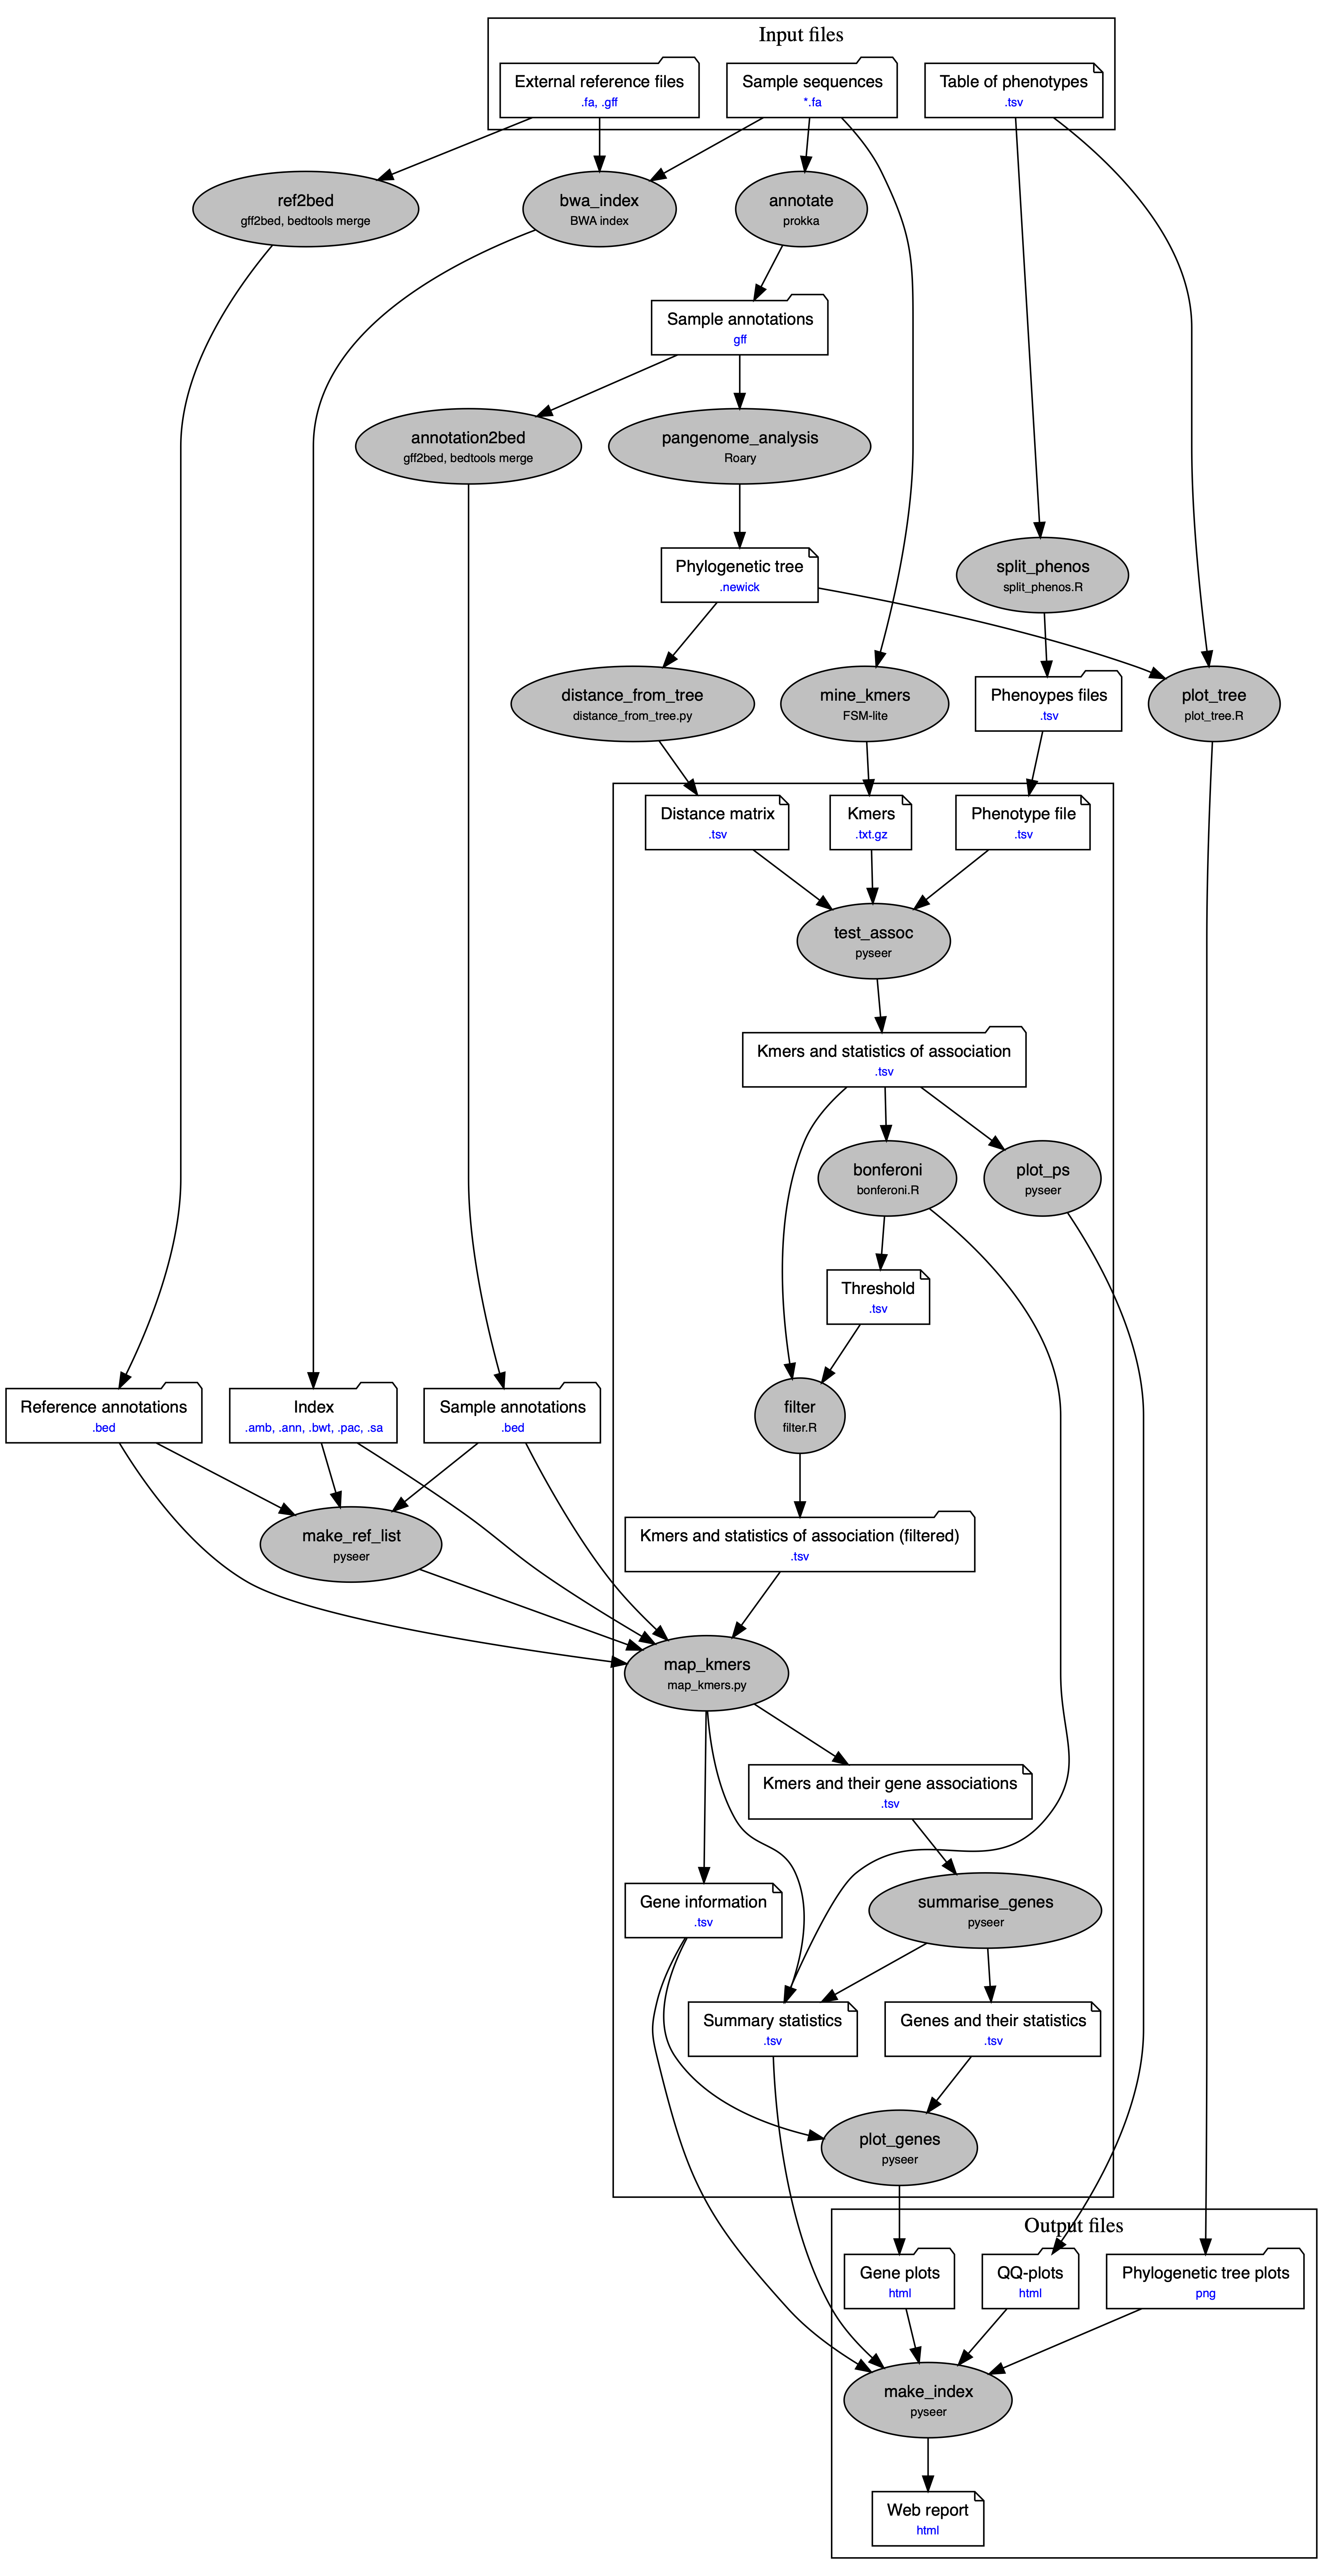
\includegraphics[height=0.9\textheight]{_static/pipe} 

}

\caption{\label{fig:pipe}Pipeline of bgwas}\label{fig:unnamed-chunk-1}
\end{figure}

\hypertarget{cgatcore}{%
\subsection{CGATcore}\label{cgatcore}}

\emph{bgwas3} was written primarily in python, utilising the piplining
framework CGATCore, (Cribbs et al. 2019), an update to CGATRuffus (ref).

The framework comes as a dependency free Python package.

The ethos behind the framework is to wrape pipeplining steps into
disperate Python functions. Through the use of python decoratiors, these
functions (referrred to as tasks)

The tool's usfulness of CGATcore is twofold.

First, the tool can make use of/ incoprtate a yml configuration file

The tool determines the dependency of tasks, and compeltes them in
order.

It checks for what tasks need to be run by files last modification
date.Therefore if files are removed or added, only tasks that are out of
date are re run.

Allows independent tasks to be run in parralel.

The recent addition (CGATCore) was written so as to take advantage of
the benefitis that computer clusters provide.

It workd alongside a Distrubuted Resourse Management Appilication API
(DRMAA) such as PBS-pri/Torque (used by imperial)

In its current iteration, \emph{bgwas3} is comprised of n `tasks', as
visualised in figure. Starting with just three file types.

\hypertarget{genome-annotation}{%
\subsection{Genome Annotation}\label{genome-annotation}}

In the \emph{bgwas} task ``annotatate'' all sample sequences are
annotated by Prokka (Seemann 2014) The tool functions as follows: It
first makes predictions on features using a number of external tools
including Prodigal {[}@{]} for the anotation of coding region, RNAmmer
for ribosomal RNA genes, Aragorn for transfer RNA genes, SignalP for
signal leader peptides and Infernal for non-coding RNA. After feature
prediction, the speculative features are queryed against a umber of
databes suchs as UniProt {[}@{]}, Refseq {[}@{]} and Pfam.

The function of annotating input sequences in the \emph{bgwas3} pipeline
is twofold. First, gene annotations are later used to estimate the
phylogenetic tree of the sample, and secondly, significantly associated
Kmers are later mapped to the annatated genomes when identifying the
Kmer's genetic identity.

\hypertarget{kmer-minig-and-counting}{%
\subsection{Kmer minig and counting}\label{kmer-minig-and-counting}}

\emph{bgwas3} integrates the tool fsm-lite (Välimäki 2018) to count
`mine' and count Kmers. of user defined variable length kmers in the all
samples. fsm-lite benefits first by being able to run on a single core,
but also because of its ability to read and count Kmers not of a single
length, but of a range of lengths, unlike similar tools such as DSK? As
mentioned before, the length of Kmers effects the specificuty and ? of
the association testing. Therefore \emph{bgwas3} allows the Kmers length
to be changed by editing the configuration yml file ?

\hypertarget{phylogeny-estimation-and-covariate-estimation}{%
\subsection{Phylogeny estimation and covariate
estimation}\label{phylogeny-estimation-and-covariate-estimation}}

\emph{bgwas3} currently takes a pangenomic approach to phylogeny
estimation; as in it consideres the relative prescence and absence of
genes in the samples as An estimated phylogenetic tree is estimated with
\emph{bgwas3} primariy utilisng the tool Roary (Page et al. 2015). In
summary, Roary determnes genes which fall within the coregeneome, and
then peforms clustering of isolates are clustered based on gene presence
in the accessory genome. An newick tree output of roary, is then
converted into a distance matrix using a pythons script from pyseer.

The single reasoning for prediciting phylogeny in the \emph{bgwas3}
pipeine is to use the distances defined in the distance matrix as
covariates int the assocation testing.

This is different to the standard method of multi-dimensional scaling
often used in human gwas and as part of the standard seer workflow. In
general, if a phylogeny is accurate, th

\hypertarget{kmer-association-testing}{%
\subsection{Kmer association testing}\label{kmer-association-testing}}

For linear mixed model assocation testing, a bgwas3 constructs a
distance matrix based on a phylogenetic tree. Assocation between kmers
and phenotypes is implemented with pyseer (Lees et al. 2018).

Specificially, pyseer is used to peform a linear mixed model using the
Fast-LMM algorithm (Lippert et al. 2011).

LMM tackle confounders in association tests by using a measure of
similarity (in this case a distance defined from a estimated
phylogenetic tree) as a random effect in a linear model.

TODO equation

Given a means of determining the hierarchichal relatedness between
samples, the mixed model is generally preffered, and has been shown in
past studies to control the inflation of p-values better (Lees et al.
2017).

\hypertarget{bonferoni-correction}{%
\subsection{Bonferoni correction}\label{bonferoni-correction}}

The output of pyseer, a list of all kmers and statistics relating to
their association to the given phenotype, are then filtered by their
p-value though bonferoni correction. The Bonferroni correction is a
multiple-comparison correction used when several dependent or
independent statistical tests, utilised to limit the number of spurious
positive tests. f multiple hypotheses are tested, the chance of a rare
event increases, and therefore, the likelihood of incorrectly rejecting
a null hypothesis (i.e., making a Type I error) increases An R script
\textbf{bonf.R} calculates a threshold p-value of which to accept an
assocated kmer as significant based on its p-value

\hypertarget{significant-kmer-mapping}{%
\subsection{Significant Kmer mapping}\label{significant-kmer-mapping}}

\begin{figure}
\centering
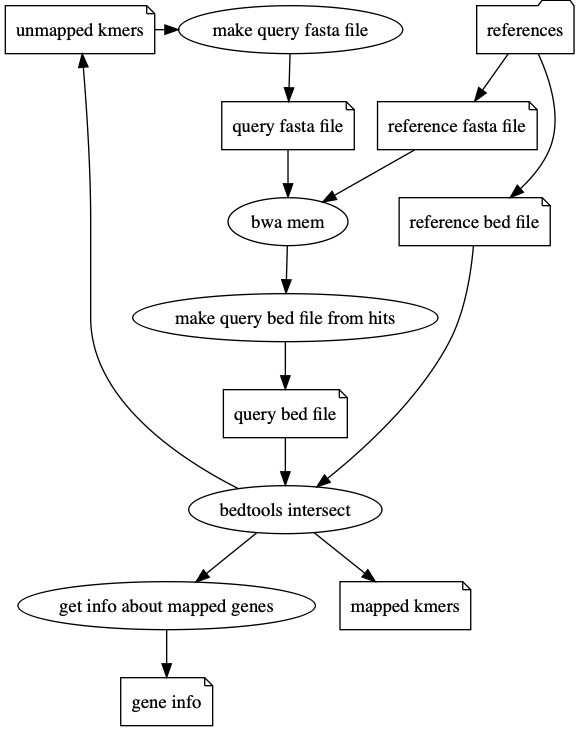
\includegraphics{_static/map_kmers.png}
\caption{\label{fig:make_kmers}Graphical representation of algorithm to
map Kmers to reference genes}
\end{figure}

A new script, written in R \textbf{map\_kmers.R}, and which calls on the
external tools BWA-Mem {[}@{]} and Bedtools {[}@{]} attempts to assign
each associated kmer to a gene found in either a supplied reference
genome, or one of the sample geneomes which has previously been
annotated. The be The script works as follows, and demonstrated in
fig:make\_kmers.

\begin{enumerate}
\def\labelenumi{\arabic{enumi}.}
\item
  Generate a Multi-Fasta file whereby all Kmers are represented as a
  single fasta enter.
\item
\end{enumerate}

\hypertarget{visualisation}{%
\subsection{Visualisation}\label{visualisation}}

An important feature of \emph{bgwas3} is the automated generation of
multiple figures, integrated into a final wbe based report.

\hypertarget{scienitif-computing-practices}{%
\subsection{Scienitif computing
practices}\label{scienitif-computing-practices}}

A significant goal of bgwas3 was to implement a useful and resuable tool
that may be used outside the scope of this singlular project.

As such, various software development principles and concepts were
applied to the project.

\hypertarget{testing-with-pytest-and-travis}{%
\subsubsection{Testing with PyTest and
Travis}\label{testing-with-pytest-and-travis}}

Pytest and

\hypertarget{documentation-with-sphinx}{%
\subsubsection{Documentation with
Sphinx}\label{documentation-with-sphinx}}

\hypertarget{packaging-with-conda}{%
\subsubsection{Packaging with Conda}\label{packaging-with-conda}}

\hypertarget{results}{%
\section{Results}\label{results}}

For the development, testing, and evaluation of \emph{bgwas3} a dataset
of

Cystic fibrosiis is a an autosomal recessive disorder that, due to a
single gene mutation, limits the ings ability to Pseaudomonas euruginosa
is one of the prmary bacteria present in the lungs of late stage and
terminal patients with cystic fibrosis. ref(Schaedel et al., 2002;
Hauser, 2011) (becomes chronic). when the lung begins to exhibit
decreased function and signs of failure For this reason, undesrstanding
the genetic adaptations pseudomonas experience when in chrnic state is
significantly important in talking this disease

This dataset involves n strains collected over a period of 24 years from
18 patients. ref

In paper () it was shown that there was `clear evidence' of the
metabolic lung environment surrounding the bacteria. Specifically
acetate production was negatively associated with length of infection
and others?

To test the usability and application of bgwas3,

The strong LD caused by the clonal reproduction of bacterial populations
means that non-causal k-mers may also appear to be associated.?

Confirmation of known resistance

\begin{longtable}[]{@{}ll@{}}
\toprule
Name & Description\tabularnewline
\midrule
\endhead
Tobromycin & Resistance to inhalant antibiotic Tobromycin\tabularnewline
Impenem & Resistance to intravenous antibiotic Imipenem\tabularnewline
Aztreonam & Resistance to intravenous/intramuscular antibiotic
Aztreonam\tabularnewline
Ciprofloxacin & Resistance to oral antibiotic
Ciprofloxacin\tabularnewline
Colistin & Resistance to `last-resort' antibioti Colistin\tabularnewline
Swim & Measure of cell surface bactera movement by
flagella\tabularnewline
Swarm & Mesaure of rapid surface movement by multiple bacteria with
rotating flagella\tabularnewline
Twitch & Measure of slow baceria movement powered by pili\tabularnewline
\bottomrule
\end{longtable}

\begin{longtable}[]{@{}l@{}}
\toprule
Chemical\tabularnewline
\midrule
\endhead
Hydrogen Cyanide\tabularnewline
Cyanide\tabularnewline
2-Furoate\tabularnewline
3-Hydroxyisovalerate\tabularnewline
3-Methylthiopropionic acid\tabularnewline
Anthranilate\tabularnewline
Betaine\tabularnewline
Cystine\tabularnewline
Formate\tabularnewline
Fumarate\tabularnewline
Histidine\tabularnewline
Isoleucine\tabularnewline
Leucine\tabularnewline
Methanol\tabularnewline
Methionine\tabularnewline
Tryptophan\tabularnewline
Uracil\tabularnewline
Valine\tabularnewline
\bottomrule
\end{longtable}

\begin{figure}
\centering
\includegraphics{report_files/figure-latex/unnamed-chunk-5-1.pdf}
\caption{\label{fig:cormat}Correlation matrix of phenotypes}
\end{figure}

\begin{figure}

{\centering 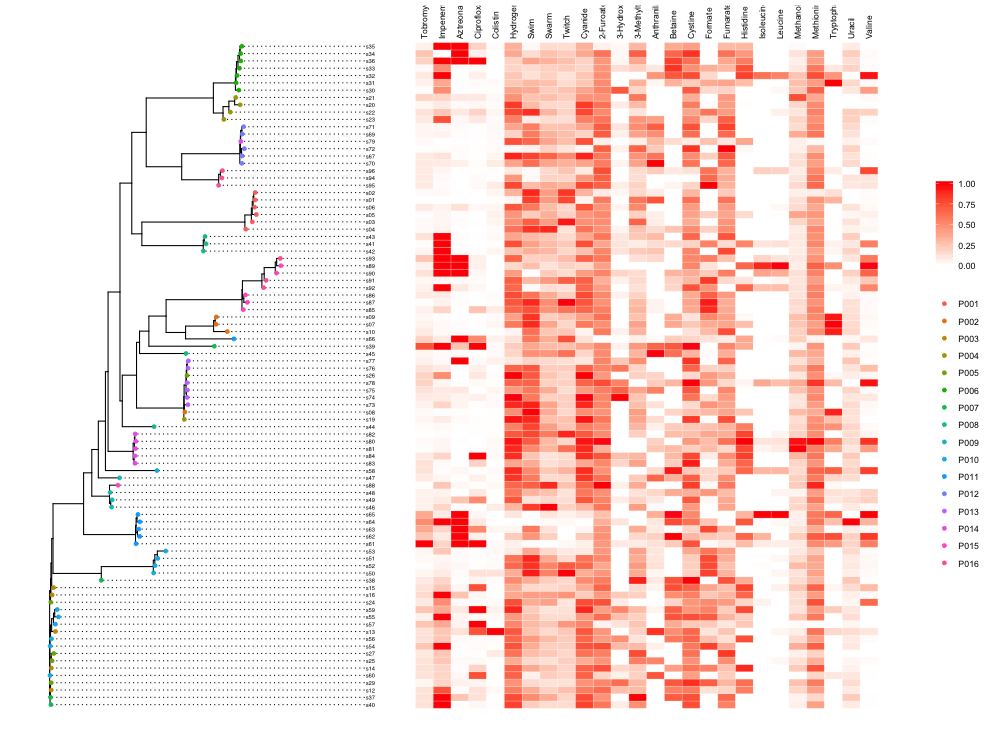
\includegraphics[height=0.9\textheight]{_static/tree} 

}

\caption{\label{fig:dens}Density plots}\label{fig:unnamed-chunk-6}
\end{figure}

\hypertarget{processing-of-phenotypes}{%
\subsection{Processing of phenotypes}\label{processing-of-phenotypes}}

\begin{figure}

{\centering 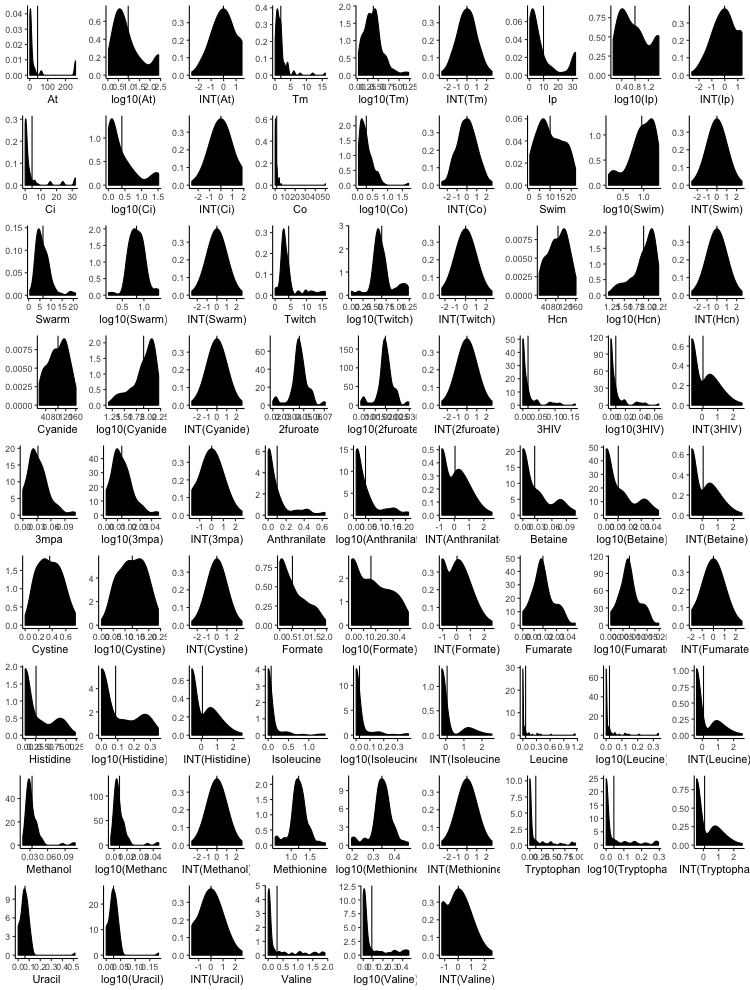
\includegraphics[height=0.9\textheight]{_static/dens} 

}

\caption{\label{fig:dens}Density plots}\label{fig:unnamed-chunk-7}
\end{figure}

When assocation testing a qualitatitve variable with linear regression,
it is generally assumed that the variable follows a normal distrubution.
Non-normal variables may fail to control for type-1 errors.

Quantitative (continuous) traits are preferred because they contain more
information. the linear regression analysis requires all variables to be
multivariate normal.

A popular statistical technique to bring normality to a continuous trait
in association studies involves peforming log transformation, or a rank
based normal transformation.

Prior to running \emph{bgwas}, the n phenotypes were seperateley log
transformed and INT, essesintially trippling the number of phenotypes
tested.

\hypertarget{annotation}{%
\subsection{Annotation}\label{annotation}}

All 91 geneomes where annotated and 14643 unique genes were identified
using Prokka.

\hypertarget{kmer-mining}{%
\subsection{Kmer mining}\label{kmer-mining}}

Number etc

\hypertarget{association-results}{%
\subsection{Association results}\label{association-results}}

\begin{figure}

{\centering 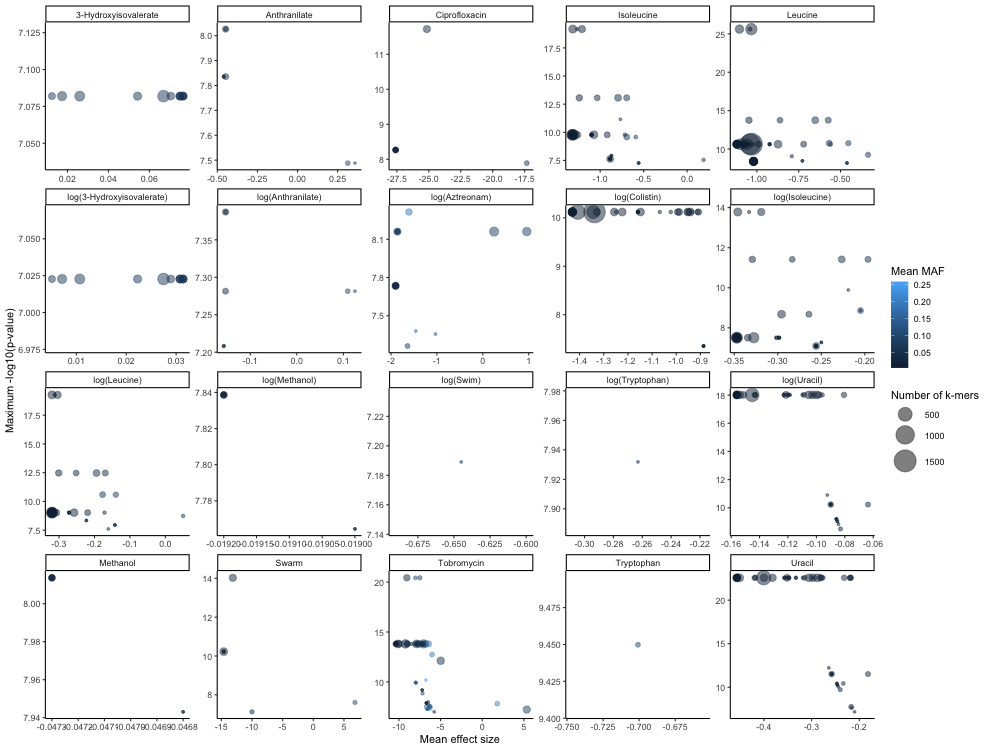
\includegraphics[height=0.9\textheight]{_static/genes} 

}

\caption{\label{fig:genes}Gens}\label{fig:unnamed-chunk-8}
\end{figure}

\begin{longtable}[]{@{}lrr@{}}
\toprule
Phenotype & Significant Kmers & Genes\tabularnewline
\midrule
\endhead
Leucine & 16450 & 289\tabularnewline
log(Colistin) & 9811 & 233\tabularnewline
Isoleucine & 5097 & 132\tabularnewline
log(Isoleucine) & 4985 & 128\tabularnewline
log(Leucine) & 4913 & 125\tabularnewline
Uracil & 2707 & 75\tabularnewline
log(Uracil) & 2470 & 72\tabularnewline
Tobromycin & 1848 & 46\tabularnewline
log(Aztreonam) & 900 & 19\tabularnewline
Ciprofloxacin & 285 & 14\tabularnewline
3-Hydroxyisovalerate & 1814 & 13\tabularnewline
log(3-Hydroxyisovalerate) & 1814 & 13\tabularnewline
Anthranilate & 210 & 7\tabularnewline
log(Anthranilate) & 210 & 7\tabularnewline
Methanol & 216 & 7\tabularnewline
log(Methanol) & 216 & 7\tabularnewline
Swarm & 229 & 7\tabularnewline
log(Swim) & 2 & 1\tabularnewline
Tryptophan & 20 & 1\tabularnewline
log(Tryptophan) & 1 & 1\tabularnewline
Aztreonam & 26891 & 0\tabularnewline
log(Ciprofloxacin) & 1 & 0\tabularnewline
log(Hydrogen Cyanide) & 1 & 0\tabularnewline
isoleucine\_int & 1 & 0\tabularnewline
\bottomrule
\end{longtable}

\hypertarget{discussion}{%
\section{Discussion}\label{discussion}}

\hypertarget{genome-annotation-1}{%
\subsection{Genome annotation}\label{genome-annotation-1}}

\hypertarget{kmer-mining-1}{%
\subsection{Kmer mining}\label{kmer-mining-1}}

The tool fsm

Prokka is a good tool ?Settings \#\# Phylogeny prediction Currently,
\emph{bgwas3} implements only a pangenomic approach approach of distance
estimation. There are other tools which involve alignment of the core
genome and snps\ldots{} May or may not be bettter Reintroduce the
problem of a large multiple alignment.

\hypertarget{references}{%
\section*{References}\label{references}}
\addcontentsline{toc}{section}{References}

\hypertarget{refs}{}
\leavevmode\hypertarget{ref-cribbs_cgat-core:_2019}{}%
Cribbs, Adam P., Sebastian Luna-Valero, Charlotte George, Ian M.
Sudbery, Antonio J. Berlanga-Taylor, Stephen N. Sansom, Tom Smith, et
al. 2019. ``CGAT-Core: A Python Framework for Building Scalable,
Reproducible Computational Biology Workflows.'' \emph{F1000Research} 8
(April): 377. \url{https://doi.org/10.12688/f1000research.18674.1}.

\leavevmode\hypertarget{ref-lees_genome-wide_2017}{}%
Lees, John A, Nicholas J Croucher, David Goldblatt, François Nosten,
Julian Parkhill, Claudia Turner, Paul Turner, and Stephen D Bentley.
2017. ``Genome-Wide Identification of Lineage and Locus Specific
Variation Associated with Pneumococcal Carriage Duration.'' Edited by
Sarah Cobey. \emph{eLife} 6 (July): e26255.
\url{https://doi.org/10.7554/eLife.26255}.

\leavevmode\hypertarget{ref-lees_pyseer:_2018}{}%
Lees, John A, Marco Galardini, Stephen D Bentley, Jeffrey N Weiser, and
Jukka Corander. 2018. ``Pyseer: A Comprehensive Tool for Microbial
Pangenome-Wide Association Studies.'' Edited by Oliver Stegle.
\emph{Bioinformatics} 34 (24): 4310--2.
\url{https://doi.org/10.1093/bioinformatics/bty539}.

\leavevmode\hypertarget{ref-lippert_fast_2011}{}%
Lippert, Christoph, Jennifer Listgarten, Ying Liu, Carl M Kadie, Robert
I Davidson, and David Heckerman. 2011. ``FaST Linear Mixed Models for
Genome-Wide Association Studies.'' \emph{Nature Methods} 8 (10):
833--35. \url{https://doi.org/10.1038/nmeth.1681}.

\leavevmode\hypertarget{ref-page_roary:_2015}{}%
Page, Andrew J., Carla A. Cummins, Martin Hunt, Vanessa K. Wong, Sandra
Reuter, Matthew T. G. Holden, Maria Fookes, Daniel Falush, Jacqueline A.
Keane, and Julian Parkhill. 2015. ``Roary: Rapid Large-Scale Prokaryote
Pan Genome Analysis.'' \emph{Bioinformatics} 31 (22): 3691--3.
\url{https://doi.org/10.1093/bioinformatics/btv421}.

\leavevmode\hypertarget{ref-seemann_prokka:_2014}{}%
Seemann, Torsten. 2014. ``Prokka: Rapid Prokaryotic Genome Annotation.''
\emph{Bioinformatics} 30 (14): 2068--9.
\url{https://doi.org/10.1093/bioinformatics/btu153}.

\leavevmode\hypertarget{ref-valimaki_fsm-lite_2018}{}%
Välimäki, Niko. 2018. ``Fsm-Lite.''
\url{https://github.com/nvalimak/fsm-lite}.


\end{document}
